\subsection*{e. Obtener el estado, segmento y el total de clientes que no han solicitado ninguna orden.}

Primero separaremos a los clientes que tienen una cuenta y no tienen una orden, de los que sí tienen una orden. Posteriormente, obtendremos los atributos de estos clientes y los agruparemos respecto a 'state' y 'segment', contando el número de clientes en cada grupo y colocándolo como una columna llamada 'numclientes'.

Expresión:
\begin{equation}
\gamma_{\text{state}, \text{segment}; \, \text{COUNT}(\text{customerid}) \to \text{numclientes}} \left( \left( \left( \pi_{\text{customerid}}(\text{customer}) - \pi_{\text{customerid}}(\text{orders}) \right) \bowtie \text{customer} \right) \right)
\end{equation}

Resultados Obtenidos:

\begin{figure}[H]
  \centering
  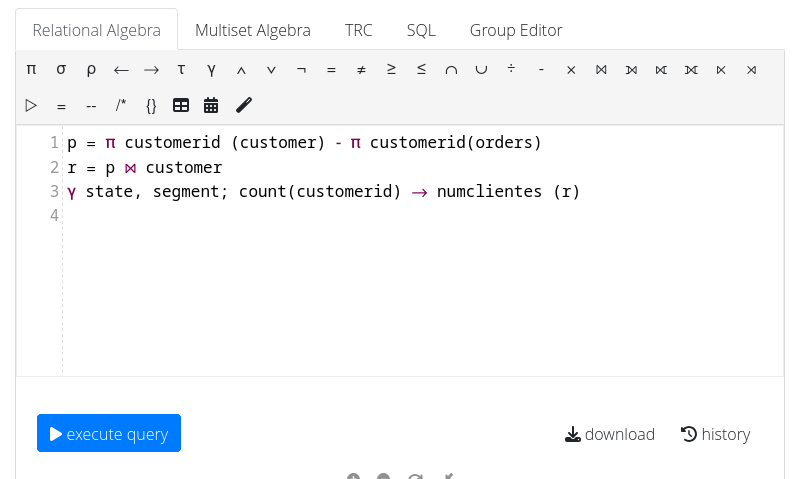
\includegraphics[width=0.7\textwidth]{imagenes/2.e-Query.png}
  \caption{Consulta}
\end{figure}

\begin{figure}[H]
  \centering
  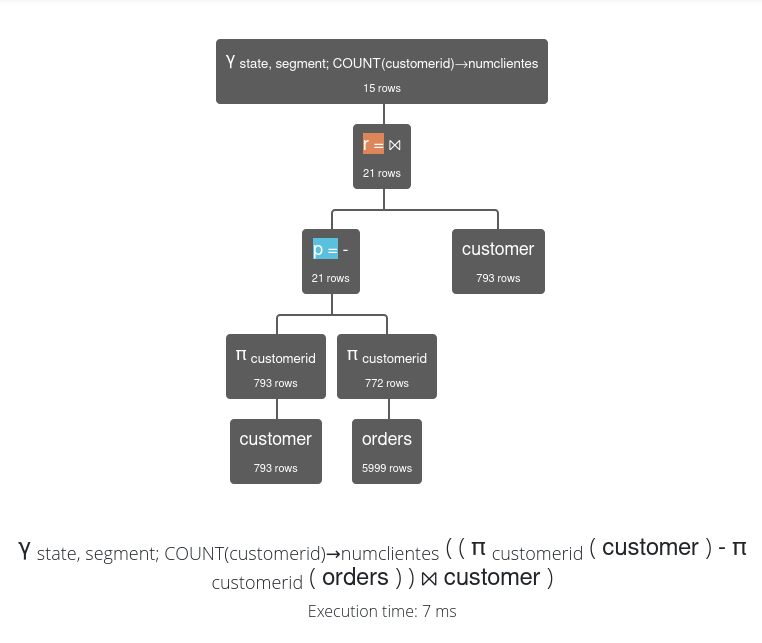
\includegraphics[width=0.7\textwidth]{imagenes/2.e-Three.png}
  \caption{Árbol de consulta.}
\end{figure}

\begin{figure}[H]
  \centering
  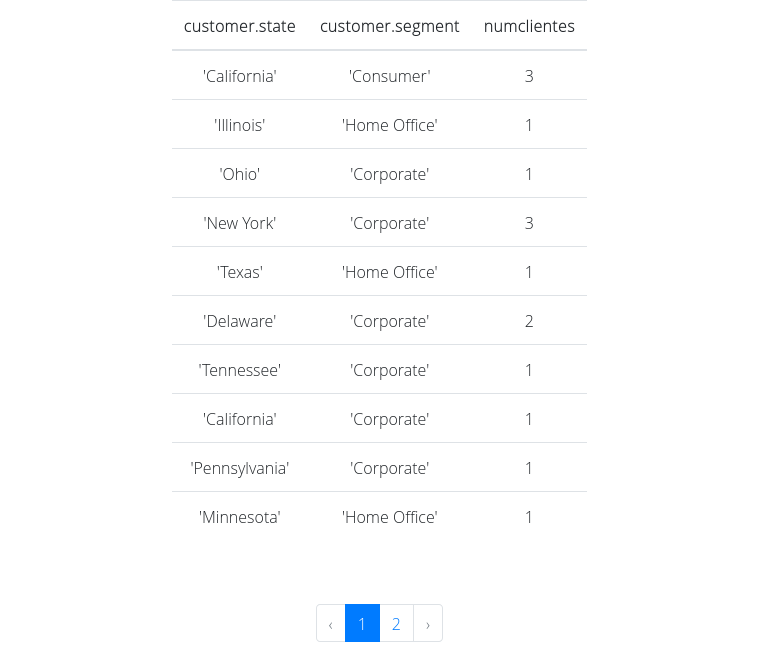
\includegraphics[width=0.7\textwidth]{imagenes/2.e-Tabla.png}
  \caption{Resultado de consulta.}
\end{figure}
